\documentclass[xcolor=dvipsnames]{beamer} % dvipsnames gives more built-in colors
\mode<presentation>

\usetheme{Boadilla}

\definecolor{GWdarkblue}{HTML}{033C5A}

\usecolortheme[named=GWdarkblue]{structure}

% Sets the font
\usepackage[defaultfam,tabular,lining]{montserrat}
\setbeamerfont{title}{shape=\scshape}
\setbeamerfont{frametitle}{shape=\scshape}
%Remove "Figure" from captions
\setbeamertemplate{caption}{\raggedright\insertcaption\par}

\usepackage{graphicx}
\usepackage{tabularx}
\usepackage{hyperref}

\usepackage{soul}
\makeatletter
\let\HL\hl
\renewcommand\hl{%
  \let\set@color\beamerorig@set@color
  \let\reset@color\beamerorig@reset@color
  \HL}
\makeatother

\title[Regression]{Regression}
\author[SMPA 2152]{Data Analysis for Journalism and Political Communication (Fall 2024)}
\date{Prof. Bell}

\begin{document}

%%%%%%%%%%%%%%%%%%%%%%%%%%%%%%%%%%%%%%%%%%%%%%%%%%%%%%%%%%%%%%%%%%
\frame{
\titlepage
}

%%%%%%%%%%%%%%%%%%%%%%%%%%%%%%%%%%%%%%%%%%%%%%%%%%%%%%%%%%%%%%%%%%
\frame{\frametitle{What is Regression?}

\begin{itemize}[<+->]
    \item So far, we've learned how to compare the mean of two groups using a \textbf{t-test}
    \item But often, a t-test is too restrictive for the analysis we want to conduct:
    \begin{itemize}
        \item What if we have two continuous variables? Income, age, and years of education are common variables that we may not want to force into two discrete categories.
        \item What about \textbf{confounders}? For example, we found that Americans allocate less money to welfare applicants who are rated as ``poor'' workers compared to ``excellent'' workers. What are some possible confounders we need to consider?
    \end{itemize}
    \item \textbf{Regression} is a set of tools that allow us to efficiently evaluate the correlation between two variables while accounting for potential confounders
\end{itemize}
}

%%%%%%%%%%%%%%%%%%%%%%%%%%%%%%%%%%%%%%%%%%%%%%%%%%%%%%%%%%%%%%%%%%
\frame{\frametitle{Introduction to Linear Regression}
\begin{itemize}[<+->]
    \item We will focus on the simplest regression method called Ordinary Least Squares (OLS), or \textbf{linear regression}
    \item Linear regression is used to estimate the effect of a change in the \textbf{independent} (explanatory) variable on the mean of the \textbf{dependent} (outcome) variable
    \item Why is it called ``linear'' regression? In practice, we are just running a best fit line through a scatter plot of two variables.
\end{itemize}
}

%%%%%%%%%%%%%%%%%%%%%%%%%%%%%%%%%%%%%%%%%%%%%%%%%%%%%%%%%%%%%%%%%%
\frame{\frametitle{Estimating the Regression (Best Fit) Line}
\only<1-3>{The linear regression equation is:
\begin{center}
$Y = \beta_0 + \beta_1X + \epsilon$\\
~\\
$Y$ = dependent variable\\
$\beta_0$ = intercept\\
$\beta_1$ = slope, also called a coefficient\\
$X$ = independent variable\\
$\epsilon$ = error
\end{center}}

\only<2-3>{This looks very similar to a linear equation you might have learned before:
\begin{center}
$y = ax + b$\\
\only<3>{$y = b + ax$}
\end{center}}

\only<4-7>{You want to estimate the effect of religiosity on political activism. The linear regression equation is:
\begin{center}
$\hat{Activism} = \hat{\beta}_0 + \hat{\beta}_1Religiosity$
\end{center}

The \enspace  $\hat{}$ \enspace is the mathematical notation for ``estimate of the mean''\\
~\\
\only<5-7>{If ``Religiosity'' has a value of 4, and the intercept is 1, and the coefficient is .5, what is our estimated mean of ``Activism''?}

\only<6-7>{\begin{center}
$\hat{Activism} = 1 + .5(4)$
\end{center}}

\only<7>{So the coefficient ($\beta_1$) is the effect of a \textbf{one-unit} change in religiosity on the mean of political activism.}
}

\only<8>{
\centering
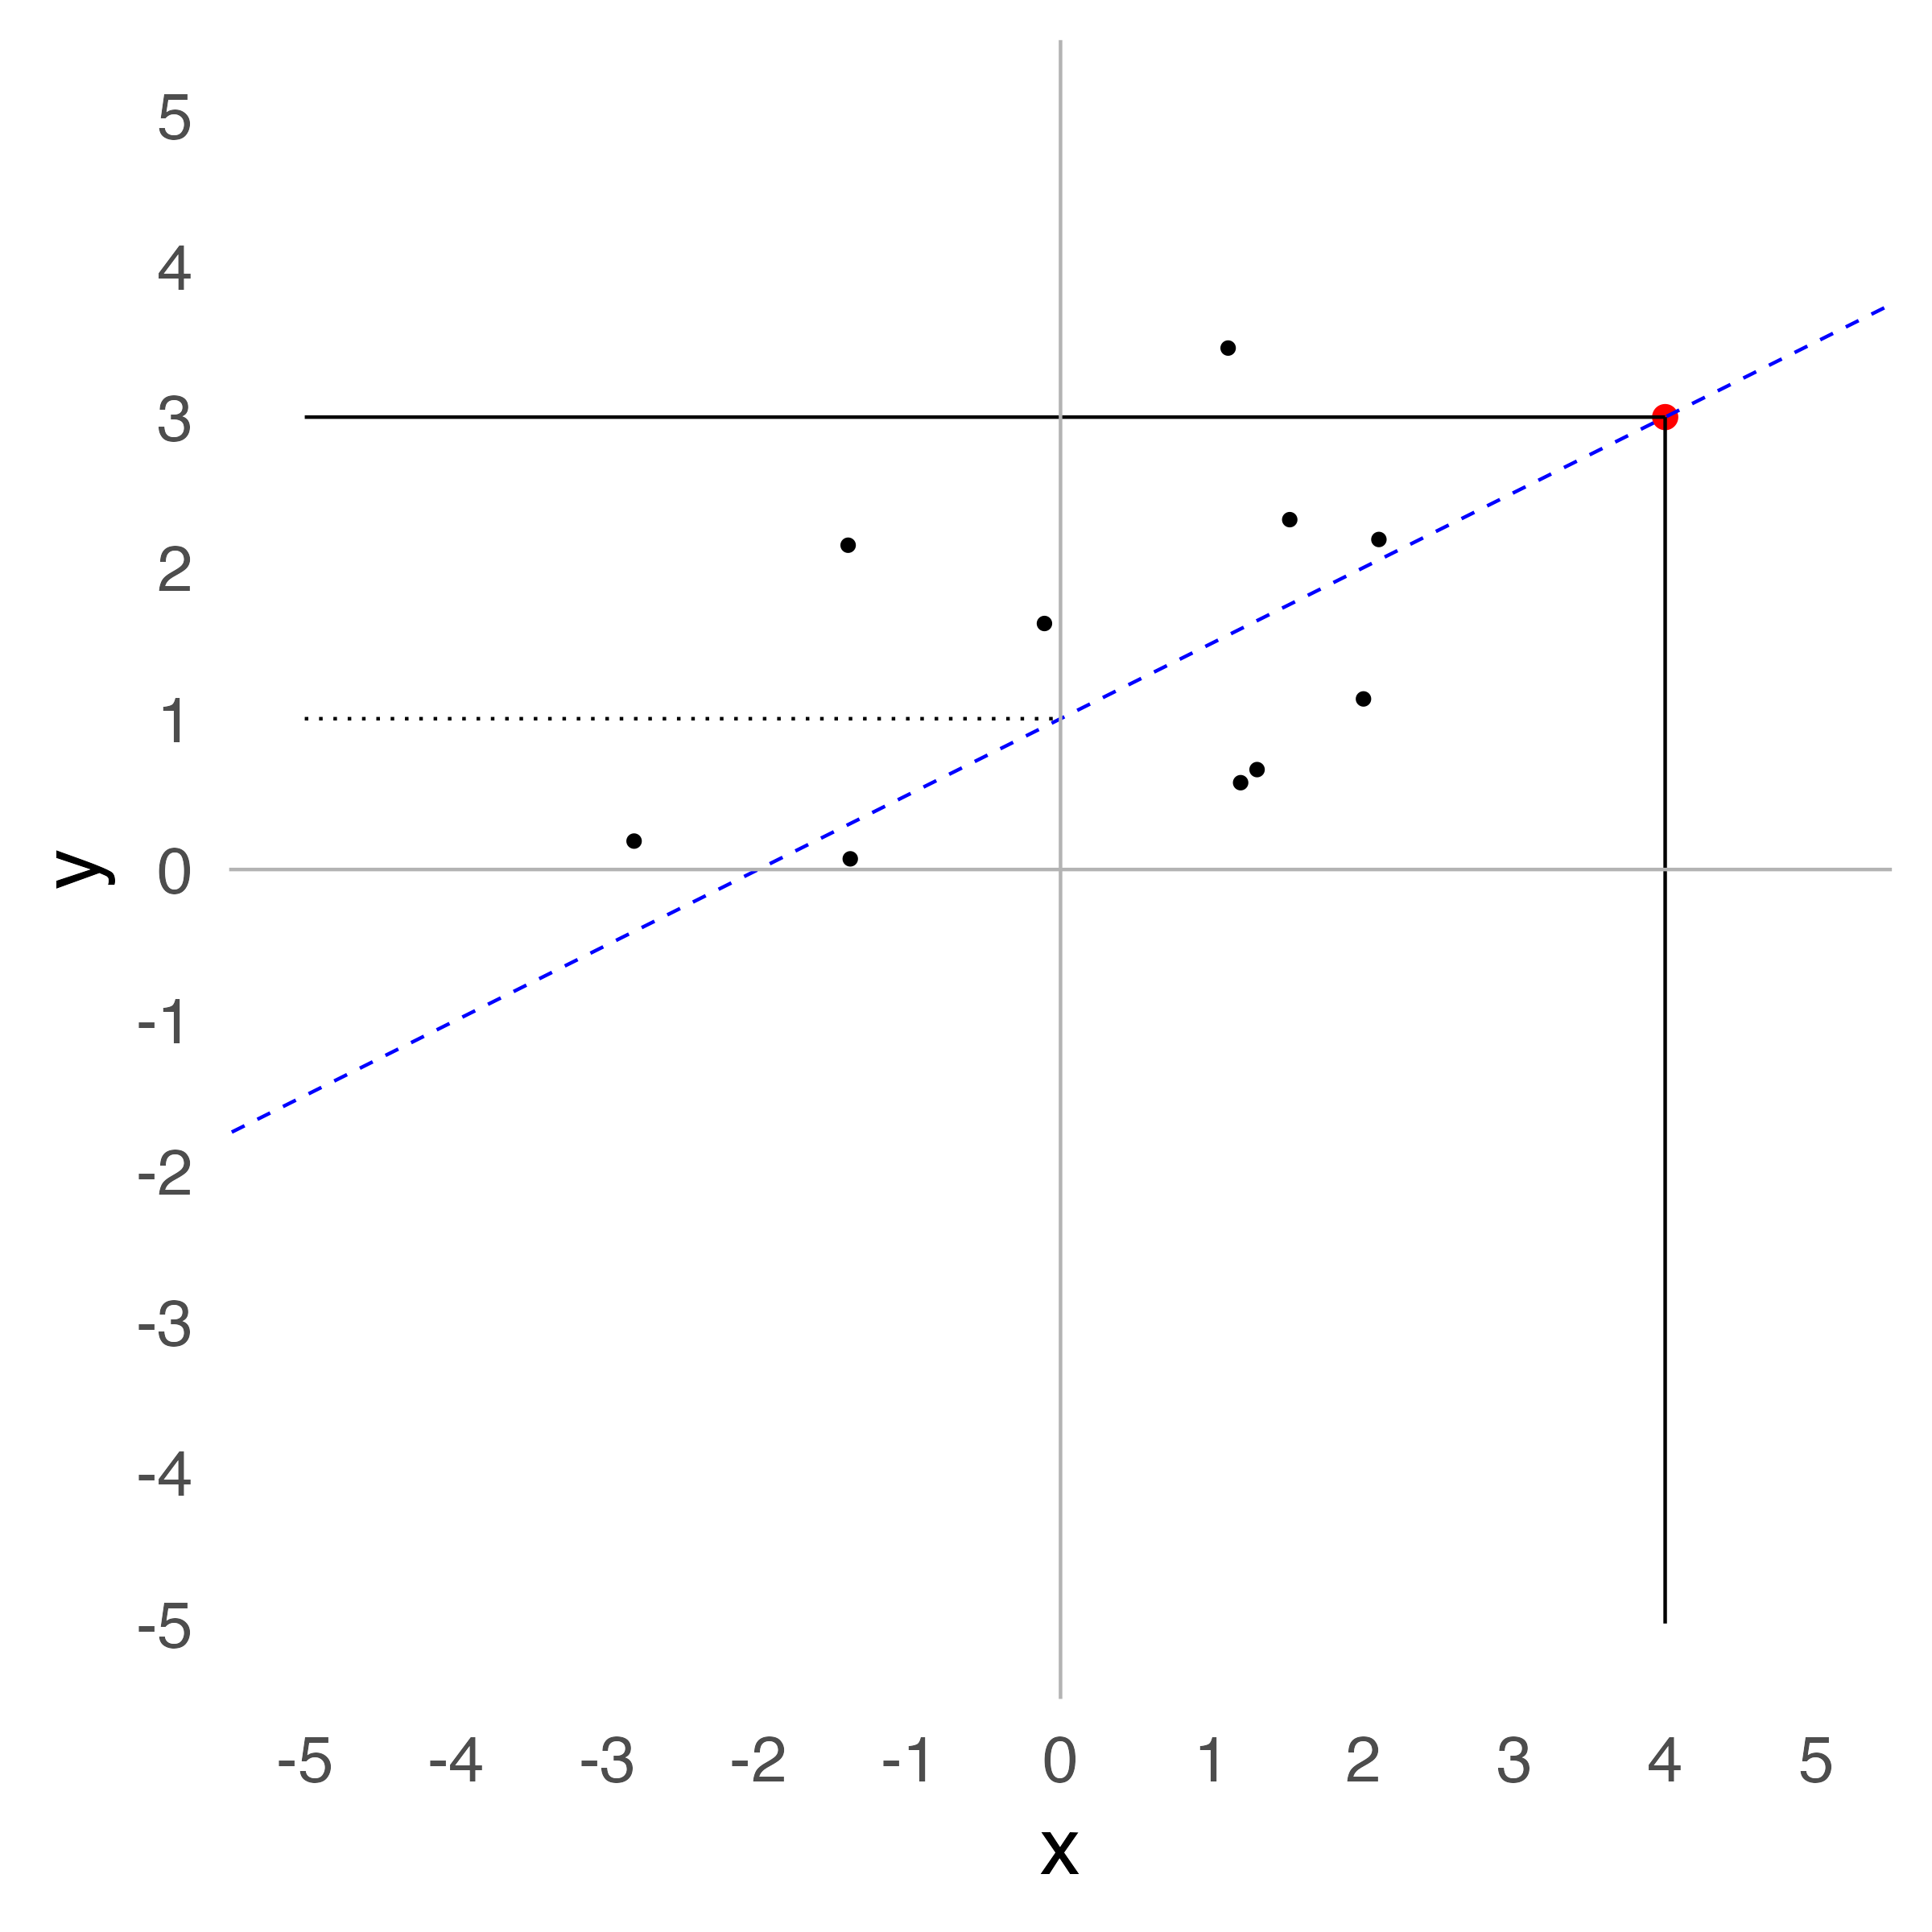
\includegraphics[height = .8\textheight]{linear_equation.png}
}
}

%%%%%%%%%%%%%%%%%%%%%%%%%%%%%%%%%%%%%%%%%%%%%%%%%%%%%%%%%%%%%%%%%%
\frame{\frametitle{What Is Error?}
\only<1>{Recall that the linear regression equation is:
\begin{center}
$Y = \beta_0 + \beta_1X + \epsilon$\\
~\\
$Y$ = dependent variable\\
$\beta_0$ = intercept\\
$\beta_1$ = slope, also called a coefficient\\
$X$ = independent variable\\
$\epsilon$ = error
\end{center}}
\only<3>{\centering
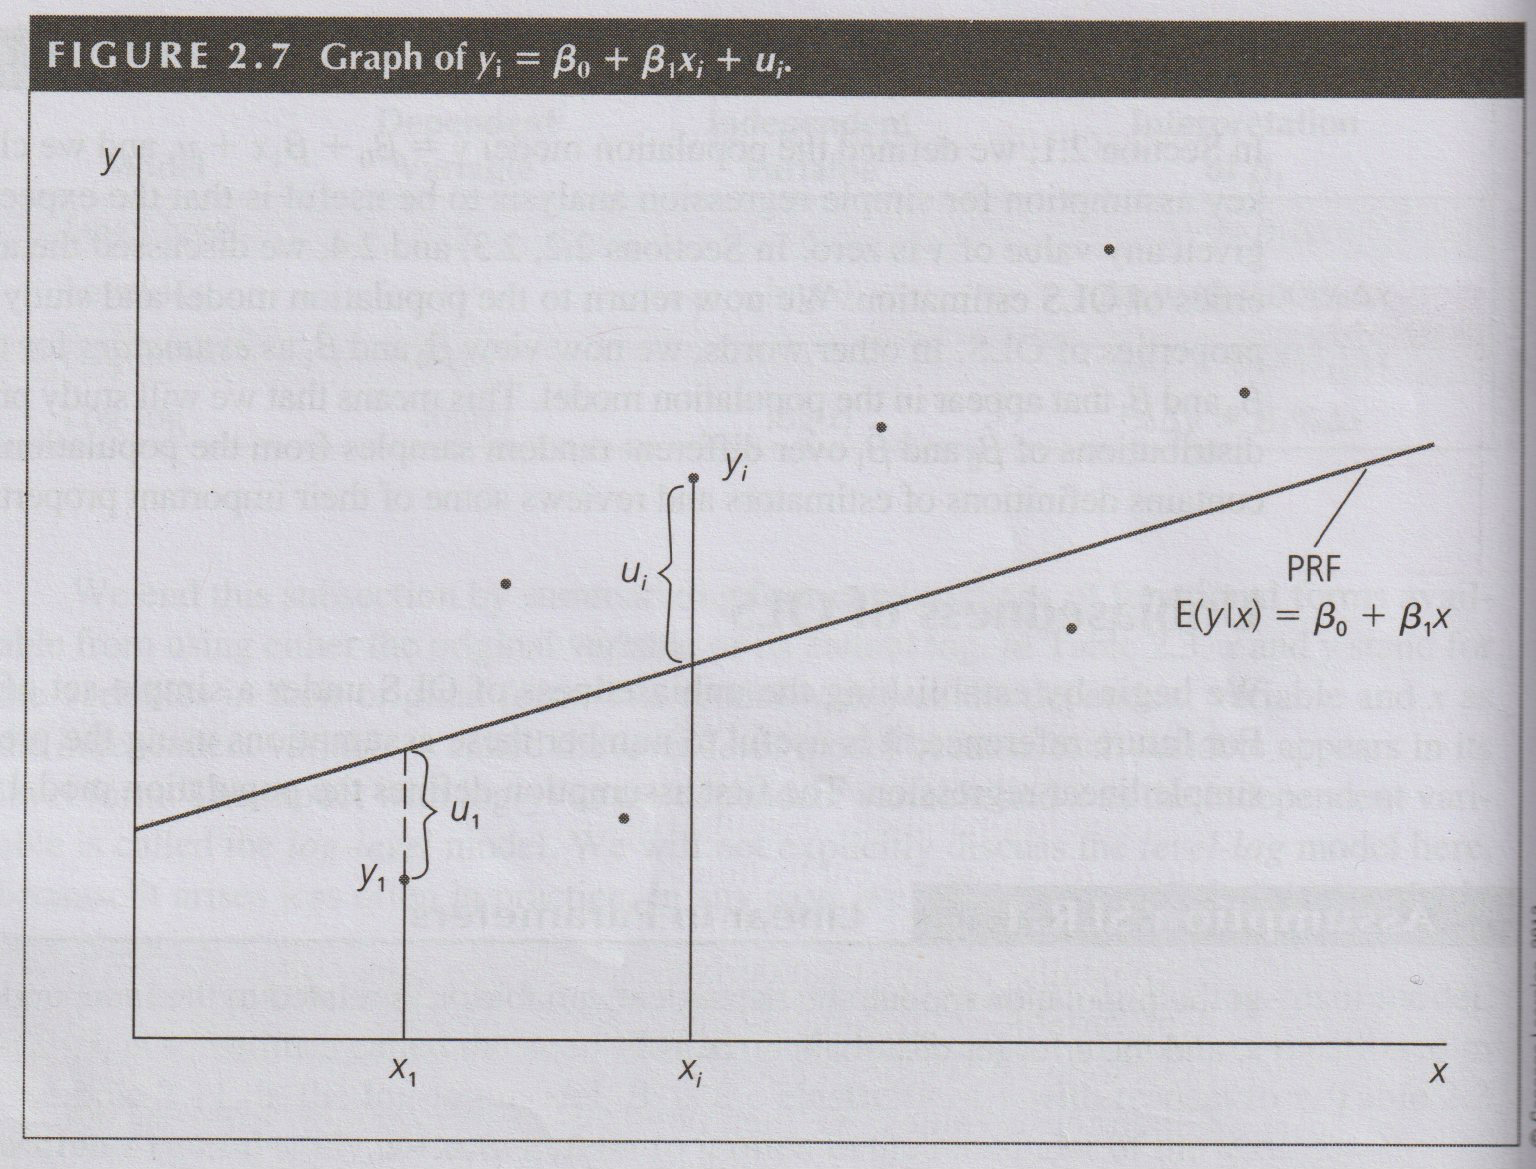
\includegraphics[width=.8\textwidth]{RegressionError.png}}
\only<2,4->{\begin{itemize}[<+->]
    \item Error ($\epsilon$ or $u$) is also called the residual (left over from $Y = \beta_0 + \beta_1X$, our best fit line)
    \item<3-> Our goal in regression is to fit the best line that  minimizes the error
    \item<5> However, we can never get the $\epsilon$ = 0, and often we don't even get close. We just do the best we can to make the ``best'' best fit line.
\end{itemize}}
}

%%%%%%%%%%%%%%%%%%%%%%%%%%%%%%%%%%%%%%%%%%%%%%%%%%%%%%%%%%%%%%%%%%
\frame{\frametitle{Multiple Linear Regression}
\only<1-3>{The multiple linear regression equation is:
\begin{center}
$Y = \beta_0 + \beta_1X_1 + \beta_2X_2 + \epsilon$\\
~\\
$Y$ = dependent variable\\
$\beta_0$ = intercept\\
$\beta_i$ = slope coefficient\\
$X_i$ = independent variable\\
$\epsilon$ = error
\end{center}
\only<2>{\textcolor{blue}{What is the interpretation of $\beta_1$?}\\
~\\
$\beta_1$ is the effect of a one-unit change in $X_1$ on the mean of $Y$, holding $X_2$ fixed (the independent effect of $X_1$ on $Y$)}
\only<3>{\textcolor{blue}{What is the interpretation of $\beta_2$?}\\
~\\
$\beta_2$ is the effect of a one-unit change in $X_2$ on the mean of $Y$, holding $X_1$ fixed (the independent effect of $X_2$ on $Y$)}}
\only<4>{\centering
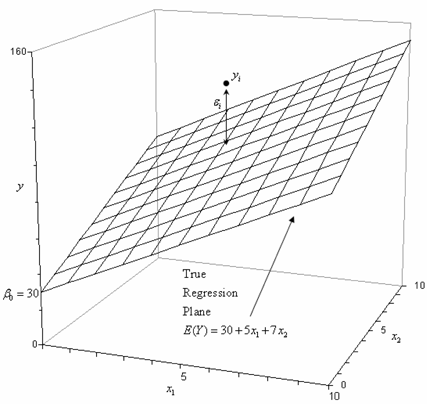
\includegraphics[width=.6\textwidth]{3dregression.png}}
}

%%%%%%%%%%%%%%%%%%%%%%%%%%%%%%%%%%%%%%%%%%%%%%%%%%%%%%%%%%%%%%%%%%
\frame{\frametitle{Example}

\only<1>{
\footnotesize
``Working Twice as Hard to Get Half as Far: Race, Work Ethic, and America’s Deserving Poor''\\
Christopher D. DeSante, \textit{Am. Journal of Political Science} vol. 57 iss. 2 (2013)
~\\
~\\
\centering
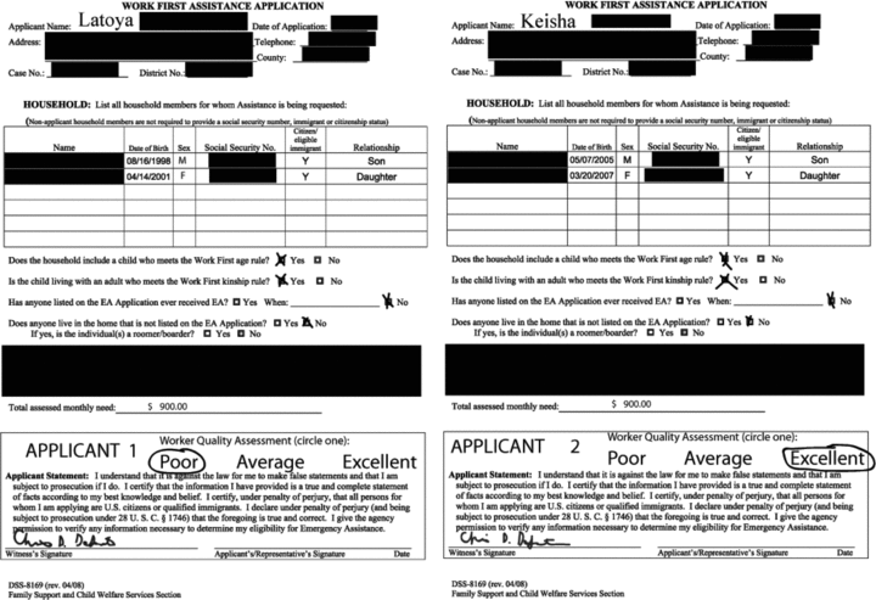
\includegraphics[height = .8\textheight]{desante_treatment.png}
}

\only<2>{\begin{center}
$\hat{Allocation} = \hat{\beta_0} + \hat{\beta_1}Race + \hat{\beta_2}WorkEthic + \hat{\beta_3}Age + \hat{\beta_4}Gender + \hat{\beta_3}PoliticalParty$
\end{center}}
}

%%%%%%%%%%%%%%%%%%%%%%%%%%%%%%%%%%%%%%%%%%%%%%%%%%%%%%%%%%%%%%%%%%
\frame{\frametitle{How Many Independent Variables?}
\begin{itemize}[<+->]
    \item Our goal is to include all of the independent variables that could plausibly affect the dependent variable
    \item But we do not include all possible variables (the kitchen sink method) because it makes our regression mathematically less efficient
    \item One way to evaluate how well you are explaining change in $Y$ is through the $R^2$, technically called the ``coefficient of determination''
    \item $R^2$ ranges from 0 to 1 and represents the proportion of change in $Y$ explained by $X_i$
    \item My pet peeve is over-relying on the $R^2$ - theory should drive your modeling decisions, not a summary statistic
\end{itemize}
}

%%%%%%%%%%%%%%%%%%%%%%%%%%%%%%%%%%%%%%%%%%%%%%%%%%%%%%%%%%%%%%%%%%
\frame{\frametitle{Non-Continuous Dependent Variables}
\begin{itemize}[<+->]
    \item One of the assumptions of linear regression is that the relationship between $X$ and $Y$ is linear (you can draw a best fit line)
    \item This assumption is usually fine when we are working with continuous dependent variables like income
    \item What about categorical dependent variables, like party ID? The linear regression model is not well suited for these.
    \item What about binary dependent variables, like support for a policy?\\
    ~\\
    We call this a linear probability model because it estimates the effect of a one-unit change in $X$ on the \textit{probability} (percent chance) of a value of ``1'' for the dependent variable
\end{itemize}
}

\end{document}
